\documentclass[../../main.tex]{subfiles}
\begin{document}

\section{Finite Elementer}

I finite element-metoden bygger vi opp funksjonsrom ved å sette sammen små byggeklosser kalt \emph{finitte elementer}. Hvert element beskriver funksjoner lokalt over et lite delområde av vårt totale domene. Dette reiser to fundamentale spørsmål:
\begin{itemize}
    \item Hvordan ser en funksjon ut over et enkelt element?
    \item Hvordan knyttes funksjoner sammen mellom elementer?
\end{itemize}

For å svare på disse spørsmålene må vi først forstå den matematiske strukturen til et finitt element.

\subsection{Ciarlet-trippel}

Et finitt element er abstrakt sett en matematisk struktur som beskrives ved en såkalt \emph{Ciarlet-trippel}, oppkalt etter Philippe G. Ciarlet. Denne trippelen spesifiserer fullstendig geometrien, funksjonene og frihetsgrader for elementet.

\begin{definition}{Ciarlet-trippel}{ciarlet-triple}
En \textbf{Ciarlet-trippel} er en triplett $(\mathcal{K}, \mathcal{P}, \mathcal{N})$ hvor:
\begin{enumerate}
    \item $\mathcal{K} \subseteq \mathbb{R}^n$ er en begrenset, lukket mengde med ikke-tomt indre og stykkevis glatt rand $\partial \mathcal{K}$ -- \emph{elementdomenet}.
    \item $\mathcal{P}$ er et endelig-dimensjonalt rom av funksjoner definert på $\mathcal{K}$ -- rommet av \emph{formfunksjoner}.
    \item $\mathcal{N} = \{N_1, N_2, \ldots, N_k\}$ er en basis for dualrommet $\mathcal{P}^\star$ -- mengden av \emph{nodale variabler} (også kalt \emph{degrees of freedom}).
\end{enumerate}
\end{definition}

\begin{remark}
Dualrommet $\mathcal{P}^\star$ består av alle lineære funksjonaler $N: \mathcal{P} \to \mathbb{R}$. De nodale variablene $N_i$ er typisk punktevalueringer (f.eks. $N_i(v) = v(z_i)$) eller deriverte (f.eks. $N_i(v) = \frac{\partial v}{\partial x}(z_i)$).
\end{remark}

\begin{remark}
Dualrommet $\mathcal{P}^\star$ består av alle lineære funksjonaler $N: \mathcal{P} \to \mathbb{R}$. De nodale variablene $N_i$ er typisk punktevalueringer (f.eks. $N_i(v) = v(z_i)$) eller deriverte (f.eks. $N_i(v) = \frac{\partial v}{\partial x}(z_i)$).
\end{remark}

\subsection{Unisolvens}

For at et finitt element skal være veldefinert, må de nodale variablene være tilstrekkelige til å bestemme funksjonen i $\mathcal{P}$ entydig. Dette konseptet kalles \emph{unisolvens}.

\begin{definition}{Unisolvens}{unisolvence}
Mengden av nodale variabler $\mathcal{N}$ \textbf{bestemmer} $\mathcal{P}$ (vi sier at $\mathcal{N}$ er \emph{unisolvent} for $\mathcal{P}$) hvis:
\[
    N(\psi) = 0 \quad \forall N \in \mathcal{N} \quad \implies \quad \psi = 0
\]
for alle $\psi \in \mathcal{P}$.
\end{definition}

\begin{remark}
Intuitivt betyr unisolvens at hvis en funksjon i $\mathcal{P}$ forsvinner på alle noder, så må funksjonen være identisk null. Dette sikrer at vi kan rekonstruere enhver funksjon i $\mathcal{P}$ entydig fra dens nodalverdier.
\end{remark}

\subsection{Nodal basis}

Gitt et finitt element $(\mathcal{K}, \mathcal{P}, \mathcal{N})$, kan vi konstruere en spesiell basis for $\mathcal{P}$ som har en enkel relasjon til de nodale variablene.

\begin{definition}{Nodal basis}{nodal-basis}
En basis $\{\phi_1, \phi_2, \ldots, \phi_k\}$ for $\mathcal{P}$ kalles en \textbf{nodal basis} hvis:
\[
    N_i(\phi_j) = \delta_{ij} = \begin{cases}
        1, & i = j \\
        0, & i \neq j
    \end{cases}
\]
for alle $i, j = 1, \ldots, k$.
\end{definition}

\begin{remark}
I en nodal basis har basisfunksjonen $\phi_j$ verdien 1 ved node $j$ og 0 ved alle andre noder. Dette gjør interpolasjon svært enkel: en vilkårlig funksjon $v \in \mathcal{P}$ kan skrives som:
\[
    v = \sum_{i=1}^k N_i(v) \phi_i
\]
\end{remark}

\begin{remark}
I en nodal basis har basisfunksjonen $\phi_j$ verdien 1 ved node $j$ og 0 ved alle andre noder. Dette gjør interpolasjon svært enkel: en vilkårlig funksjon $v \in \mathcal{P}$ kan skrives som:
\[
    v = \sum_{i=1}^k N_i(v) \phi_i
\]
\end{remark}

\subsection{Eksempel: Endimensjonalt element}

La oss se på det enkleste eksemplet på et finitt element.

\begin{example}{Endimensjonalt Lagrange-element}{1d-element}
La $\mathcal{K} = [a, b]$ være et intervall, $\mathcal{P} = \mathbb{P}_q$ være rommet av polynomer av grad høyst $q$, og la $\mathcal{N} = \{N_0, N_1, \ldots, N_q\}$ hvor:
\[
    N_i(v) = v\left(a + \frac{(b - a)i}{q}\right), \quad \forall v \in \mathcal{P}, \quad i = 0, 1, \ldots, q
\]
De nodale variablene evaluerer altså funksjonen på $q+1$ jevnt fordelte punkter i intervallet.

Siden $\dim(\mathbb{P}_q) = q+1 = |\mathcal{N}|$, og nodene bestemmer polynomet entydig (unisolvens), er dette et gyldig finitt element.
\end{example}

\begin{center}
    \input{figures/02/1D-element.tikz}
\end{center}

\begin{center}
    \input{figures/02/1D-element.tikz}
\end{center}

\subsection{Matematisk verktøy: Hyperplan og dekonstruksjonslemmaet}

For å bevise at mer komplekse elementer tilfredsstiller unisolvens, trenger vi noen matematiske verktøy. Spesielt viktig er konseptet med hyperplan og det såkalte \emph{dekonstruksjonslemmaet}.

\begin{definition}{Hyperplan}{hyperplane}
Et \textbf{hyperplan} i $\mathbb{R}^n$ er mengden av punkter $x \in \mathbb{R}^n$ som tilfredsstiller en lineær ligning:
\[
    L(x) = 0
\]
hvor $L: \mathbb{R}^n \to \mathbb{R}$ er en ikke-triviell lineær funksjon.
\end{definition}

\begin{remark}
I $\mathbb{R}^2$ er et hyperplan en linje, i $\mathbb{R}^3$ er det et plan. Vi misbruker notasjonen ved å referere til både funksjonen $L$ og mengden $\{x : L(x) = 0\}$ som \emph{hyperplanet}.
\end{remark}

\begin{lemma}{Dekonstruksjonslemmaet (DL)}{deconstruction-lemma}
La $P$ være et polynom av grad $d = \deg(P) \geq 1$ som forsvinner på hyperplanet $L$ (dvs. $P(x) = 0$ for alle $x$ slik at $L(x) = 0$). Da kan $P$ faktoriseres som:
\[
    P = L \cdot Q
\]
hvor $Q$ er et polynom av grad $\deg(Q) = d - 1$.
\end{lemma}

\begin{lemma}{Dekonstruksjonslemmaet (DL)}{deconstruction-lemma}
La $P$ være et polynom av grad $d = \deg(P) \geq 1$ som forsvinner på hyperplanet $L$ (dvs. $P(x) = 0$ for alle $x$ slik at $L(x) = 0$). Da kan $P$ faktoriseres som:
\[
    P = L \cdot Q
\]
hvor $Q$ er et polynom av grad $\deg(Q) = d - 1$.
\end{lemma}

\begin{proof}
Uten tap av generalitet antar vi at $L(x) = x_n$ (hvor $x = (x_1, \ldots, x_{n-1}, x_n) \in \mathbb{R}^n$), det vil si at hyperplanet er beskrevet av $\{x : x_n = 0\}$.

Vi skriver $x = (\hat{x}, x_n)$ hvor $\hat{x} = (x_1, \ldots, x_{n-1})$ og $\hat{i} = (i_1, \ldots, i_{n-1})$ er en multi-indeks. Siden $\deg(P) = d$ kan vi skrive:
\[
    P(\hat{x}, x_n) = \sum_{j=0}^d \sum_{|\hat{i}| \leq d - j} C_{\hat{i}j} \hat{x}^{\hat{i}} x_n^j
\]

Siden $P$ forsvinner på hyperplanet, har vi $P(\hat{x}, 0) = 0$ for alle $\hat{x}$:
\[
    P(\hat{x}, 0) = \sum_{|\hat{i}| \leq d} C_{\hat{i}0} \hat{x}^{\hat{i}} = 0
\]

Dette impliserer at alle koeffisientene $C_{\hat{i}0} = 0$ for alle multi-indekser $\hat{i}$ med $|\hat{i}| \leq d$. Dermed kan vi omskrive $P$ som:
\[
    P(\hat{x}, x_n) = \sum_{j=1}^d \sum_{|\hat{i}| \leq d - j} C_{\hat{i}j} \hat{x}^{\hat{i}} x_n^j = x_n \underbrace{\sum_{j=1}^d \sum_{|\hat{i}| \leq d - j} C_{\hat{i}j} \hat{x}^{\hat{i}} x_n^{j-1}}_{Q(\hat{x}, x_n)}
\]

Vi har dermed $P = x_n \cdot Q = L \cdot Q$ hvor $\deg(Q) = d - 1$.
\end{proof}

\section{Triangulære elementer}

Vi ser nå på de mest brukte finite elementene i to dimensjoner: triangulære elementer. Disse bygger på trekanter som elementdomener.

\subsection{Lineære Lagrange-elementer}

Det enkleste og mest grunnleggende todimensjonale finite elementet er det lineære Lagrange-elementet.

\begin{definition}{Lineært Lagrange-element}{linear-lagrange-element}
La $\mathcal{K}$ være en trekant med hjørner $z_1, z_2, z_3$. Det \textbf{lineære Lagrange-elementet} er definert ved:
\begin{itemize}
    \item $\mathcal{P} = \mathbb{P}_1$, rommet av polynomer av grad høyst 1 i to variabler.
    \item $\mathcal{N} = \{N_1, N_2, N_3\}$ hvor $N_i(v) = v(z_i)$ for $i = 1, 2, 3$.
\end{itemize}
Merk at $\dim(\mathbb{P}_1) = 3$, så antallet nodale variabler matcher dimensjonen til funksjonsrommet.
\end{definition}

\begin{center}
 \input{figures/02/linear-lagrange-element-1.tikz}
\end{center}

I figuren representerer $\cdot$ nodene $z_i$ og $L_i$ representerer kantene (kanten motsatt hjørne $i$).

\begin{proof}[Bevis at $\mathcal{N}$ bestemmer $\mathbb{P}_1$ (unisolvens)]
La $L_1, L_2, L_3$ være lineære funksjoner som beskriver kantene til trekanten $\mathcal{K}$, det vil si $L_i = 0$ på kant nummer $i$.

Anta at $P \in \mathbb{P}_1$ tilfredsstiller $N_i(P) = 0$ for $i = 1, 2, 3$, det vil si $P$ forsvinner på alle tre hjørnene.

Siden $P$ er lineær i to variabler, er restriksjonen $P|_{L_1}$ et lineært polynom i én variabel langs kanten $L_1$. Dette polynomet forsvinner på to punkter (hjørnene $z_2$ og $z_3$), og det eneste lineære polynomet med to nullpunkter er nullpolynomet. Dermed har vi $P|_{L_1} \equiv 0$.

Ved dekonstruksjonslemmaet \ref{lem:deconstruction-lemma} kan vi skrive $P = L_1 \cdot c$ hvor $c$ er en konstant (siden $\deg(P) = 1$ impliserer $\deg(c) = 0$).

Men $P(z_1) = 0$ og $L_1(z_1) \neq 0$ (siden $z_1$ ikke ligger på kant $L_1$), så:
\[
    P(z_1) = c \cdot L_1(z_1) = 0 \quad \implies \quad c = 0
\]

Derfor er $P \equiv 0$, og vi konkluderer med at $\mathcal{N}$ bestemmer $\mathbb{P}_1$.
\end{proof}

\begin{remark}
Valget av hjørnepunktene som noder er ikke unikt, men det er den mest naturlige og brukte konfigurasjonen. Et annet gyldig valg kunne for eksempel vært å bruke midtpunktene på kantene som noder.
\end{remark}

\begin{center}
    \input{figures/02/linear-lagrange-element-2.tikz}
\end{center}

\begin{example}{Triangulært element av $\mathbb{P}_2$}{p2-triangle-element}
    La $\mathcal{K}$ være en trekant, $\mathcal{P}_2$ være mengden av polynomer (i to variabler) av grad $\deg(P) \leq 2$ og $\mathcal{N} = \{N_1, N_2, N_3, N_4, N_5, N_6\}$ hvor:
    \[
        N_i(v) =
        \begin{cases}
             & v(z_i), \quad i = 1, 2, 3 \text{ (vertices) }           \\
             & v(z_i), \quad i = 4, 5, 6 \text{ (midpoints of edges) }
        \end{cases}
    \]
    \begin{center}
        \input{figures/02/p2-triangle-element.tikz}
    \end{center}

    For å bekrefte at dette er et finite element må vi sjekke at $\mathcal{N}$ bestemmer $\mathcal{P}_2$:

    Anta $P \in \mathcal{P}_2$ forsvinner på alle noder $z_i$. Siden $P|_{L_1}$ er kvadratisk i én variabel og forsvinner på $3$ punkter, må $P|_{L_1} = 0$.

    Ved \emph{(DL)} har vi
    \[P = L_1 Q_1\]
    med
    \[\deg(Q_1) = \deg(P) - 1 = 1\]

    Siden
    \[P|_{L_2} = 0\]
    har vi
    \[L_1Q_1|_{L_2} = 0\]
    So
    \[Q_1|_{L_2} = 0 \text{ (a.e.)} \text{ since } L_1(z_1) \neq 0\]

    except possible at $z_3$.

    By continuity of $Q_1$ we have
    \[Q_1|_{L_2} = 0\]

    Applying \emph{(DL)} again we find
    \[Q_1 = L_2 Q_2, \text{ with } \deg(Q_2) = \deg(Q_1) - 1 = 0 \implies Q_2 = c\]
    and that
    \[P = c L_1 L_2\]
    Observe that $P(z_6) = 0$ and is not on $L_1, L_2$, so:
    \[P(z_6) = c L_1(z_6) L_2(z_6) = 0 \implies c = 0\]
    since
    \[L_1(z_6), L_2(z_6) \neq 0\]

    Thus $P \equiv 0$ and $\mathcal{N}$ determines $\mathcal{P}_2$, so it is a finite element.\qed

\end{example}

\section{Lecture 12: 25.09.2025}
\begin{example}{General Lagrange element}{}
    \[
        \mathcal{N}_k = \{N_i\}_{i=1}^{\frac12(k+1)(k+2)}, \quad
        N_i =
        \begin{cases}
            3 \text{ Vector Nodes}             \\
            3(k-1) \text{ Distinct Edge Nodes} \\
            \frac12(k-1)(k-2) \text{ Interior Nodes}
        \end{cases}
    \]
    With interior points chosen to determine $\mathbb{P}_k$.

    Let $k=3$ for the moment:

    \begin{center}
        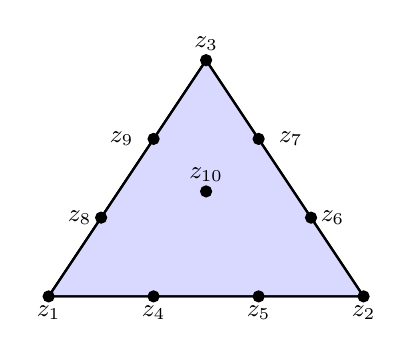
\begin{tikzpicture}[font=\small]
            \draw[thick, fill=blue!50, fill opacity=0.3] (0, 0) -- (4, 0) -- (2, 3) -- cycle;
            \draw[thick] (0, 0) -- (4, 0) -- (2, 3) -- cycle;
            \node[below] at (0, 0) {$z_1$};
            \node[below] at (4, 0) {$z_2$};
            \node[above] at (2, 3) {$z_3$};
            % Edge nodes for k=3: two per edge
            \node[below] at (1.333, 0) {$z_4$};
            \node[below] at (2.667, 0) {$z_5$};
            \node[right] at (3.333, 1) {$z_6$};
            \node[right] at (2.8, 2) {$z_7$};
            \node[left] at (0.667, 1) {$z_8$};
            \node[left] at (1.2, 2) {$z_9$};
            % Interior node
            \node[above] at (2, 1.333) {$z_{10}$};

            \filldraw[black] (0, 0) circle (2pt);
            \filldraw[black] (4, 0) circle (2pt);
            \filldraw[black] (2, 3) circle (2pt);
            \filldraw[black] (1.333, 0) circle (2pt);
            \filldraw[black] (2.667, 0) circle (2pt);
            \filldraw[black] (3.333, 1) circle (2pt);
            \filldraw[black] (2.667, 2) circle (2pt);
            \filldraw[black] (0.667, 1) circle (2pt);
            \filldraw[black] (1.333, 2) circle (2pt);
            \filldraw[black] (2, 1.333) circle (2pt);
        \end{tikzpicture}
    \end{center}

    For $k=4$:
    \begin{center}
        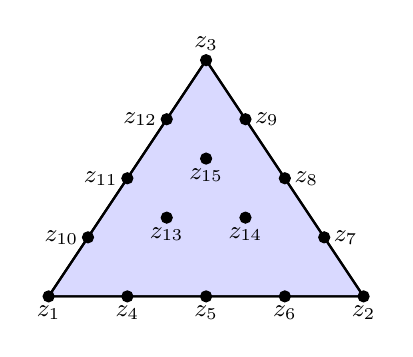
\begin{tikzpicture}[font=\small]
            \draw[thick, fill=blue!50, fill opacity=0.3] (0, 0) -- (4, 0) -- (2, 3) -- cycle;
            \draw[thick] (0, 0) -- (4, 0) -- (2, 3) -- cycle;
            \filldraw[black] (0, 0) circle (2pt) node[below] {$z_1$};
            \filldraw[black] (4, 0) circle (2pt) node[below] {$z_2$};
            \filldraw[black] (2, 3) circle (2pt) node[above] {$z_3$};
            % Edge nodes for k=4: three per edge
            \filldraw[black] (1, 0) circle (2pt) node[below] {$z_4$};
            \filldraw[black] (2, 0) circle (2pt) node[below] {$z_5$};
            \filldraw[black] (3, 0) circle (2pt) node[below] {$z_6$};
            \filldraw[black] (3.5, 0.75) circle (2pt) node[right] {$z_7$};
            \filldraw[black] (3, 1.5) circle (2pt) node[right] {$z_8$};
            \filldraw[black] (2.5, 2.25) circle (2pt) node[right] {$z_9$};
            \filldraw[black] (0.5, 0.75) circle (2pt) node[left] {$z_{10}$};
            \filldraw[black] (1, 1.5) circle (2pt) node[left] {$z_{11}$};
            \filldraw[black] (1.5, 2.25) circle (2pt) node[left] {$z_{12}$};

            % Interior nodes
            \filldraw[black] (1.5, 1) circle (2pt) node[below] {$z_{13}$};
            \filldraw[black] (2.5, 1) circle (2pt) node[below] {$z_{14}$};
            \filldraw[black] (2, 1.75) circle (2pt) node[below] {$z_{15}$};
        \end{tikzpicture}
    \end{center}
    The interior point makes a $\mathbb{P}_1$ element that is a triangle.\footnote{The proof is left as an exercise for the reader.}
\end{example}

\subsection{The Cubic Hermite}
Let $\mathcal{P} = \mathbb{P}_3$, where $\cdot$ be a point evaluation and $\odot$ a derivative evaluation, then the FE is given by $\mathcal{N} = \{N_1, \dots, N_10\}$

Abridged version to skip some technical details:

Showing this is an FE by assuming $p \in \mathbb{P}_3$ s.t.
\[
    N_i(p) = 0 \quad \forall \, i
\]

Restricting to $L_1$ then:
\[
    \begin{cases}
         & p(z_2)= p'(z_2) = 0  \\
         & p(z_3) = p'(z_3) = 0
    \end{cases}
\]
where the derivative is along the edge.
\begin{center}
    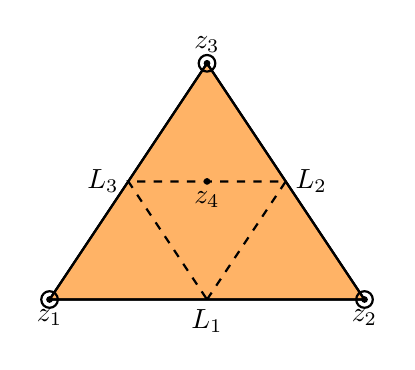
\begin{tikzpicture}
        \draw[thick, fill=orange, fill opacity=0.6] (0, 0) -- (4, 0) -- (2, 3) -- cycle;
        \draw[thick] (0, 0) -- (4, 0) -- (2, 3) -- cycle;
        \draw[thick, dashed] (2,0) -- (3, 1.5) -- (1,1.5) -- cycle;
        \draw[thick] (0, 0) circle (3pt) node[below] {$z_1$};
        \draw[thick] (4, 0) circle (3pt) node[below] {$z_2$};
        \draw[thick] (2, 3) circle (3pt) node[above] {$z_3$};
        \filldraw (2, 1.5) circle (1pt) node[below] {$z_4$};
        \filldraw (0, 0) circle (1pt);
        \filldraw (4, 0) circle (1pt);
        \filldraw (2, 3) circle (1pt);

        % Include labels for edges L_i
        \node[below] at (2, 0) {$L_1$};
        \node[right] at (3, 1.5) {$L_2$};
        \node[left] at (1, 1.5) {$L_3$};
    \end{tikzpicture}
\end{center}

The only cubic polynomial with 4 roots is $0$: $p\lvert_{L_1} \equiv 0$ and the same follows for $p\lvert_{L_2}$ and $p\lvert_{L_3}$.

By (DL) we have:

\[
    \begin{aligned}
        p        & = c L_1 L_2 L_3    &                        \\
        L_i(z_4) & \neq 0             & i = 1,2,3              \\
        p(z_4)   & = 0 \implies c = 0 & \implies \boxed{p = 0}
    \end{aligned}
\]
For a more complete proof one has to show in detail that $p = L_i Q_i$ and that if $p(x) = 0$ and $L_i \neq Q_i$ (a.e.).

\subsection{Defining the derivatives}
we need two points to derive the derivatives at a point.
In practice one might use directional derivatives.
Then the Hermite element can be drawn as follows (where the arrows is its derivative):

\begin{center}
    \begin{tikzpicture}
        \draw[thick, fill=blue!50, fill opacity=0.4] (0, 0) -- (4, 0) -- (2, 3) -- cycle;
        \filldraw[black] (0, 0) circle (2pt) node[below] at (0, 0) {$z_1$};
        \filldraw[black] (4, 0) circle (2pt) node[below] at (4, 0) {$z_2$};
        \filldraw[black] (2, 3) circle (2pt) node[above] at (2, 3) {$z_3$};
        \draw[->, thick, spaceblack] (0,0) -- (1,0);
        \draw[->, thick, spaceblack] (0,0) -- (0,1);
        \draw[->, thick, spaceblack] (4,0) -- (5,0);
        \draw[->, thick, spaceblack] (4,0) -- (4,1);
        \draw[->, thick, spaceblack] (2,3) -- (3,3);
        \draw[->, thick, spaceblack] (2,3) -- (2,4);


        % Include labels for edges L_i
        \node[below] at (2, 0) {$L_1$};
        \node[right] at (3, 1.5) {$L_2$};
        \node[left] at (1, 1.5) {$L_3$};
    \end{tikzpicture}
\end{center}
\textbf{In general} the Hermite elements have $\frac12(k+1)(k+2) \, DoF = \# \, Nodes$  where the nodal variables are:
\[
    N_i =
    \begin{cases}
        3 \text{ Vertices}    \\
        6 \text{ Derivatives} \\
        3(k-3) \text{ Edges}  \\
        \frac12(k-2)(k-1) \text{ Interior}
    \end{cases}
\]

% The Hermite element is not usually preferedover Lagrange
% but are an alt choice
% Example quintic Argyris Let D Ps in two variables and consider the
% 21 dimP dof where are pointevaluation and are istand2ⁿᵈderivati
% are normal derivatives at midpoint mi
% The proof is left as an exercise for the reader
% Proof in BS book

% To build a FE space we piece the elements together
% Def local interpolent for a FE 39,8 ur let i i k
% be the basis of N abasis for D
% The local interpolant is
% I v Nilu di
% Note v must be well defined Ni
% Eksample Consider spanned by the basisfunctions
% 1010 11,01
% 4,1 11 I y The interpolant is
% 926.9
% 9,6cg I Irv N Vaio 1 1 N VG.DE
% Vlan I
% As before the interpolant is invariant under composition
% Ikt Iq
% some more definitions
% Def Subdevision of a domain or is a finite collection
% of dement domain Ki
% s.t.int
% Ki nint Kj if itj the empty domain
% and µ K I
% Def A triangelization is a subderision where no ventet of any
% triangle lies in the interior of an edge of another triangle
% vertecis can share information
% edges can not
% ok not ok
% as ventet
% toutches an
% edgeDef Interpolant Let or have some triangelazation T of KPN
% the FE fixingm to the highest orde derivative in the nodal
% variables we can define the interpolant of a function fee a
% It
% Eit KIET
% µ
% To build a conforming FES we need to enforce conditions between
% elements Enforcing C continuity we can obtain a FES VG ECMER
% elements Through enforcing continuity the Lagrange and
% Hamite elements are a subspace of C
% C elements Enforcing C continuity the Argyri's elements are
% a subspace of C
% Let's Focus on Lagrange elements
% Det Diameter Given a set 5 diamCs 11 911
% Def Mesh conditions Let a be given and Ta be a family of
% triangulations sit
% max diam T Te Tu h diamle for och El
% further define B sit for any ET the closed convex hull
% of UB is contained in T
% We must work within convex shapes
% The family of meshes is quasi uniform if 79 0 sit
% min dium B TE Ta ghdiamler COD
% The family is non degenerate if 75 SO s t
% TE Tu and 410,1
% diamLB 2g diam T

\end{document}